\chapter{Poroelastic natural coatings}

\section{Biomimetics of poroelastic coatings}

Usually when someone is asked to imagine some "rapid" object as an airplane, a boat or a car, the common sense lead us to think about it as the smoothest as possible and most of the time shiny.
But if we look around us the nature seems not to agree with the previous statement.
In fact most of the surfaces in nature are not smooth at all, they present almost always some kind more or less regular arrangement of discontinuities at various length scales.
Since Nature have had a very large time-span to optimize this kind of surfaces we can be very certain that they are the best possible option.
One should pinpoint that the non smoothness of these surfaces can be connected to some other biological functions rather than pure fluid dynamic performance, and of course it can be the case.


With that in mind we want to show to the reader some of the most notably examples of "natural" aerodynamically surfaces.

Probably the most notable example is the shark skin, in figure \ref{fig:shark} a segment of the skin is depicted as if appears to be under the microscope.

\begin{figure}[h]
	\centering
	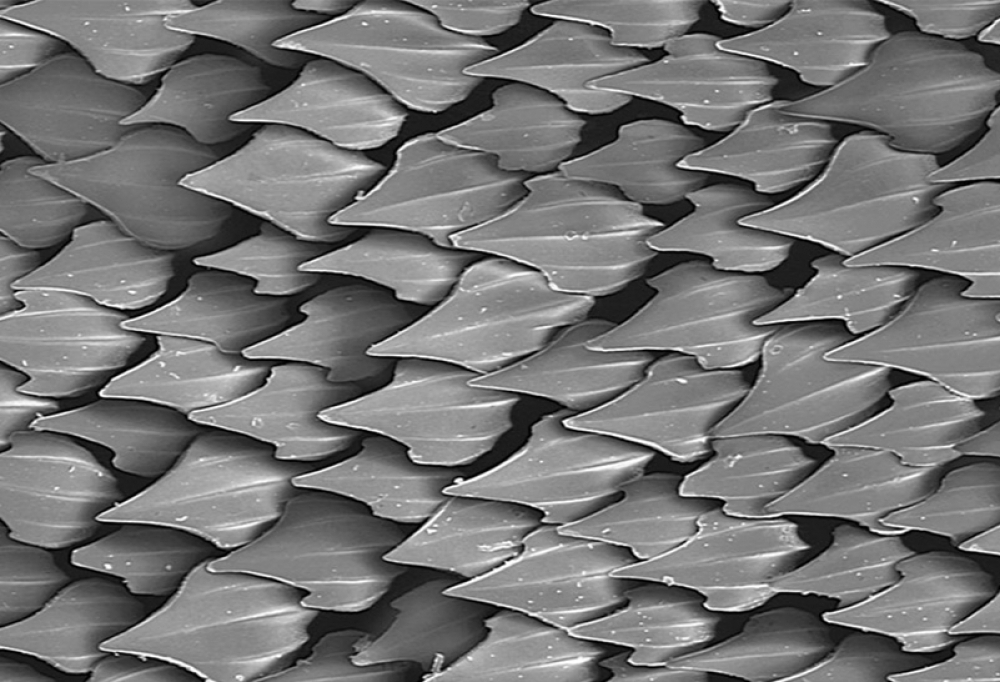
\includegraphics[width=0.6\linewidth]{chapter_1/shark}
	\caption{Microscope enlarged picture of the shark skin.}
	\label{fig:shark}
\end{figure}

The enlargement show that the surface is made up by a series of overlapped denticles, and experiment shows that they can move and interact with the flow.

The shark technology has somehow been applied by Speedo$^{\circledR}$ in their famous swimming suits, that had break multiples world records.
But it seems that this controversial swimmers performance came more on the compressed and streamlined body shape than from the surface texture itself.
In fact during the years this texture material has been publicized to be like synthetic shark skin but \cite{Oeffner785} has shown that the texture is somehow different from the shark dermal structure.
They have also performed some swimming experiment with a flat plate with different surfaces and they have found no significant speed enhancement with the swimsuit surfaces; but the measurements with the shark skin on the contrary give an appreciable improvement in the performance.


Poroelastic surfaces find also applications in aeroacoustics, in fact the owl is well known for its particularly silent flight, in the high frequency spectrum.
This characteristic is crucial for the owl in order to be able to capture his preys.
Obviously it has inspired the scientific community to study the feathers configuration and their shape.

\begin{figure}[h]
	\centering
	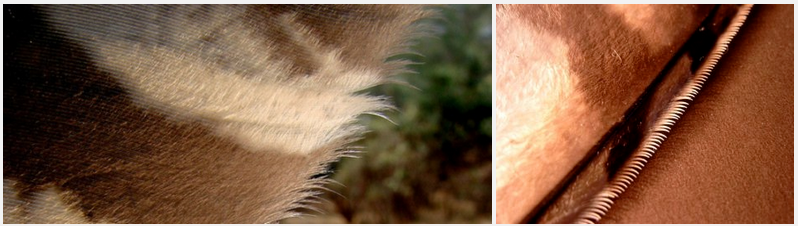
\includegraphics[width=0.8\linewidth]{chapter_1/howl}
	\caption{Feathers in owl's wing: trailing edge (left), leading edge (right). The difference in shape, and mechanical properties as rigidity, between the leading and trailing edge is a consequence of the different flow regimes in the wing.}
	\label{fig:owl}
\end{figure}
 
Multiple authors show promising result in characterizing the acoustic properties of the owl skin and their physical mechanism.
In particular \cite{lilley1998} present three main characteristic of the owl that can suppress its airborne noise: the feathers leading edge shaped like a comb, the feathers trailing edge that form a fringe and the presence of multiple "filaments" in the bottom surface of the wing and on its legs.
in the same work he also present some experimental and empirical evidence on the aeroacoustics mechanism behind the three elements above.

Another examples of work in the field of owls acoustic is the one by \cite{jaworski2013aerodynamic} in which the authors study the acoustic scattering problem of a poroelastic half-plane hit by an incident plane wave.
This configuration has been used as an analogy with the owl wing, it try to explain how the properties of this surface can suppress the noise.
They conclude that the combined effects of elasticity and porosity can produce the weakest edge noise amplification.

Recent computational simulation made by \cite{rao2017owl} confirm that the leading edge shape of the feathers truly suppress noise and enhance the lift generation for angles of attack grater then $15^{\circ}$.


Bioinspired aerodynamic surfaces include another peculiar example in the butterflies wings.
In figure \ref{fig:butterfly} the surface of a "Peacock butterfly" is enlarged in order to show the multiple scales involved; the wing structure present firstly as overlapped scales similar to the shark, but looking closely we can observe that the singles scales have a complicated permeable structure.

\begin{figure}[h]
	\centering
	\begin{subfigure}[b]{0.3\textwidth}
		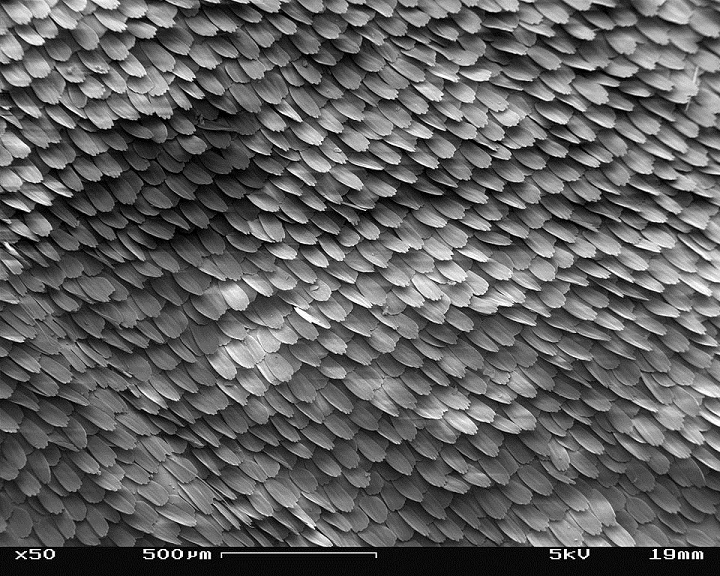
\includegraphics[width=\textwidth]{chapter_1/butterfly}
		\caption{Magnification 50x}
		\label{fig:b50}
	\end{subfigure}
	~ %add desired spacing between images, e. g. ~, \quad, \qquad, \hfill etc. 
	%(or a blank line to force the subfigure onto a new line)
	\begin{subfigure}[b]{0.3\textwidth}
		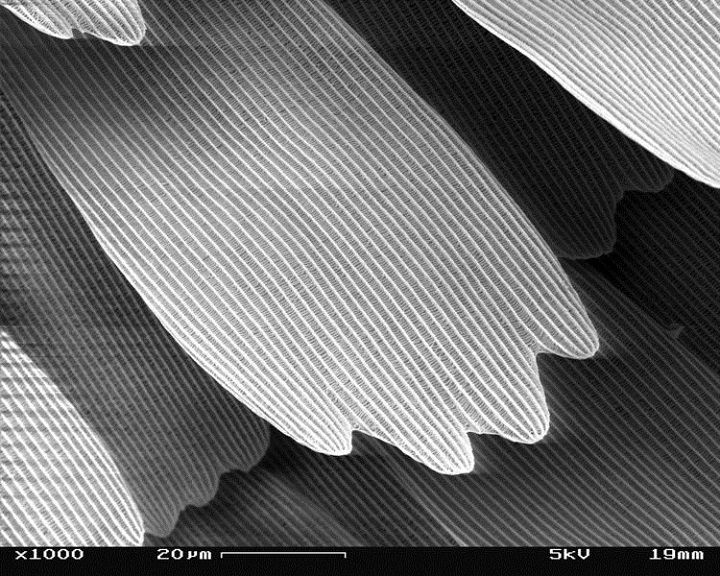
\includegraphics[width=\textwidth]{chapter_1/butterfly2}
		\caption{Magnification 1000x}
		\label{fig:b1000}
	\end{subfigure}
	\begin{subfigure}[b]{0.3\textwidth}
		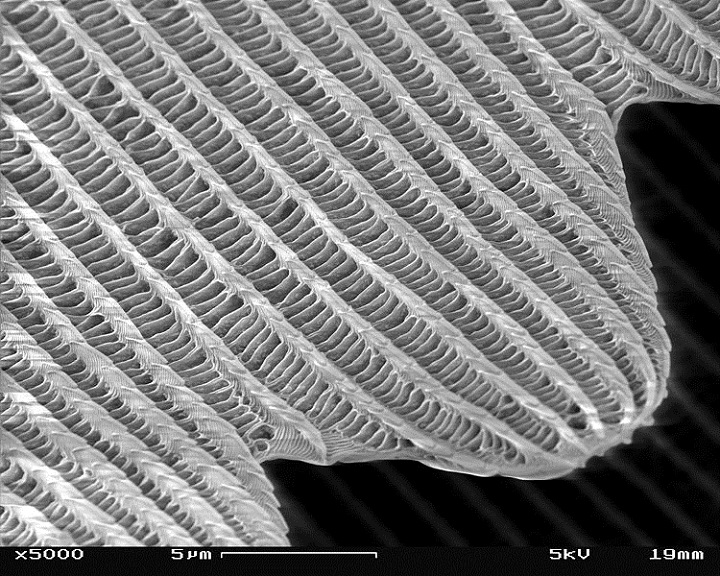
\includegraphics[width=\textwidth]{chapter_1/butterfly3}
		\caption{Magnification 5000x}
		\label{fig:b5000}
	\end{subfigure}
	\caption{Peacock butterfly wing surface using Scanning Electron Microscopy.  Images from wikimedia.org}
	\label{fig:butterfly}
\end{figure}

The work of \citet{slegers2017beneficial} the authors study the effect of such porous structure in the flight performance of butterflies.
Using cameras to measure the kinematics of their flight, they can compute their efficiency to "climb" (generate lift) and the stroke amplitude and frequency.
The authors conclude, after the proper statistical tests on the overall butterfly population, that the porous structure of their wing gives a boost in climbing efficiency about $30\%$; that results clearly stress out the importance of the poroelastic layer of the wings. 
Even though the flight aerodynamic is extremely complex \cite{srygley2002unconventional}, it seems clear that the peculiar structure of the wings surface is critical for their aerodynamic performances.


Superhydrophobic surfaces works as they were water repellent, in fact over such surfaces the water can slide over with much less resistance resulting in very small values of wettability.
This behavior is caused by the microscopic structure that forms the surface \ref{fig:lotus}, in fact the rugosities are arranged in a more or less regular way in order to be able to capture air pockets that rest inside this structures.
These air inclusion provoke an effective slip at the air-liquid interface that cause the drag reduction; but they also change the contact angle of droplets 
The work of \citet{bottaro2003effect} summarize the above aspect and their applications.

\begin{figure}[h]
	\centering
	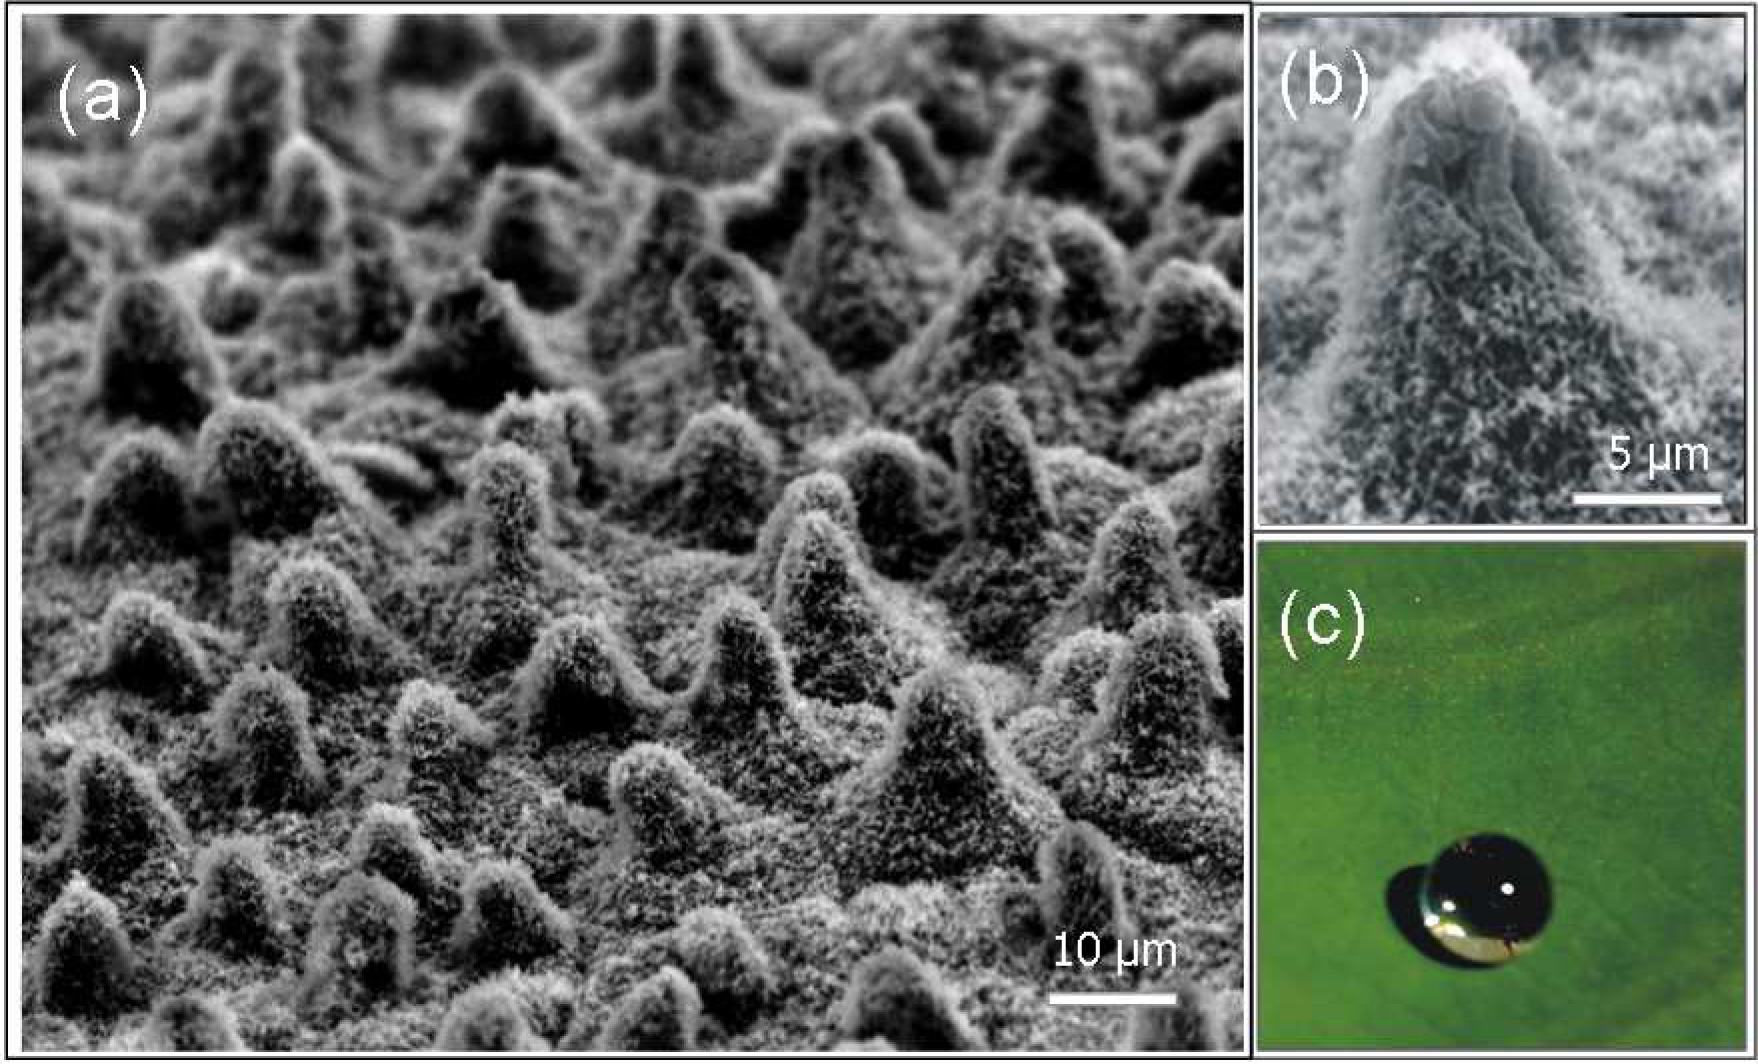
\includegraphics[width=0.6\linewidth]{chapter_1/lotus}
	\caption{(a) Scanning electron microscopy (SEM) image showing the structure of lotus leaf, (b) higher order of magnification on the single protuberance forming the surface and (c) a water drop that due to the contact angle attain an almost spherical shape. Images from \cite{stratakis2009laser}}
	\label{fig:lotus}
\end{figure}


The interest reader could find other examples and broaden the above key aspect also in \cite{bhushan2016biomimetics}, \cite{tropea2012nature}.



\subsection{Riblets and shark-skin surfaces}

We have seen that natural surface can be an inspiration to find strategies to solve many aerodynamics problems; in the following we will focus especially on the drag reduction.

Is known that the total drag contribution can be separated in different components, and the classical decomposition is between viscous drag (sometimes referred as skin friction) and pressure drag.

\begin{equation}
 \int_{A_{\sigma}}  [ \underbrace{\left( \frac{p}{\rho} \mathbf{I} \right) \cdot  \mathbf{n}_{\sigma} }_\text{pressure drag}  +  \underbrace{ \left( \nu \nabla \mathbf{v} \right) \cdot  \mathbf{n}_{\sigma}}_\text{viscous drag} ] \; dA,
 \label{eq:force}
\end{equation}

Where $A_{\sigma}$ is the solid interface of some body where a no slip condition is applied, and $ \mathbf{n}_{\sigma}$ is its outward normal.
In this section we will talk about the existing possible ways to reduce the viscous part of the drag since historically has attract more interest and/or make more progress.

In the following we will refer as the wall shear stress in the turbulent case as:
\begin{equation}
\tau = \left( \left( \mu + \mu_t \right)  \nabla \mathbf{\overline{v}} \right) \cdot  \mathbf{n}_{\sigma} = \left( \mu + \mu_t \right) \derp{\overline{u}}{y}
\end{equation}

where $\mu_t$ is the turbulent viscosity and $\overline{u}$ is the average velocity stramwise component; in the laminar case obviously the definition rest the same with some correction (there is no turbulent viscosity and no notion of average velocity).
Also $\mathbf{n}_{\sigma} = (0,1,0)$ is the conventional orientation in the literature.

Most of the industrial application involves turbulent flow; obviously there is a lot of research that aim to reduce the skin-friction in this regime.
Table 6.3.1 in the book of \citet{mclean2012understanding} make a wide list of technique already been proposed on the problem.

As the same author pinpoint the most effective, and probably the most practicable concept, are the riblets.
They are regularly arranged alternating ridges aligned in the streamwise flow direction as the figure \ref{fig:riblets1} show.

These surfaces are capable of align the turbulent flow in the mean flow direction smoothing the fluctuation of the cross-flow in the viscous sublayer.
Reducing this fluctuations close to the surface the turbulent momentum transfer will also be reduced and so the shear stress, causing the reduction in skin-friction.

\begin{figure}[h]
	\centering
	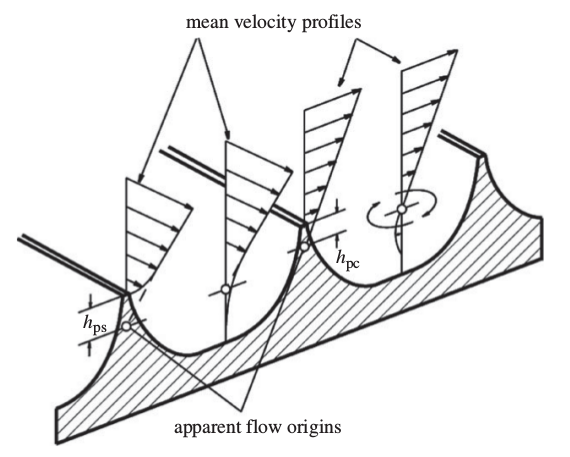
\includegraphics[width=0.7\linewidth]{chapter_1/riblets3}
	\caption{Schematics of the concept of \textit{protusion height}. The mean velocity profiles for the streamwise and crossflow velocities are presented. Where they are in the presence of a ridge is it possible to extrapolate the point of zero velocity from the velocity gradient outside the riblet, finding respectively the \textit{streamwise protusion height} $h_{ps}$ and the \textit{crossflow protusion height} $h_{pc}$. Image from \citet{bechert1997experiments}}
	\label{fig:riblets1}
\end{figure}


The viscous drag reduction correlates well with the spacing between the ridges expressed in wall units $ s^+ $, the typical shape is depicted in \ref{fig:riblets_perf} where the vertical axis show the drag reduction computed against the smooth surface case against the $ s^+ $.
This general shape of the curve, in which the skin friction decrease in certain range of spacing and then increase as the $ s^+ $ increase, is caused by a competition between the capacity of riblets to obstruct lateral fluid flow and an increase in the penetration of high speed vorticies inside this manufactured rugosities.

\begin{figure}[h]
	\centering
	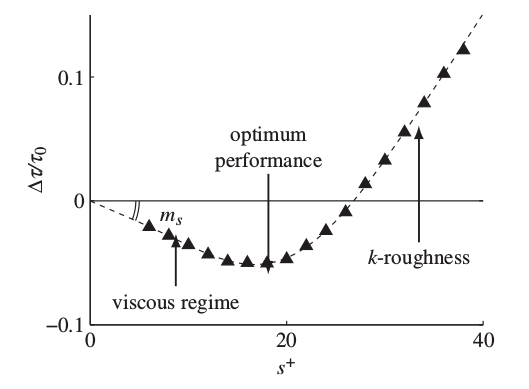
\includegraphics[width=0.5\linewidth]{chapter_1/riblets_performance}
	\caption{Performance ... \citet{jimenez2001turbulent} }
	\label{fig:riblets_perf}
\end{figure}

This last physical explanation of the riblets performances is presented in the schematics \ref{fig:riblets_schem}, where the grey areas show high skin-friction regions caused by the downwash motion generated by the near-wall vortices.
Is it clear that when the riblets are too big the vortices can penetrate inside its groove and actually increase the skin-friction due to larger area exposed to the local velocity.
On the contrary when the riblets are smaller, the high speed vortices "touch" only the tip of the ridges so only a small local area of the surface experience high-shear stresses.

\begin{figure}[h]
	\centering
	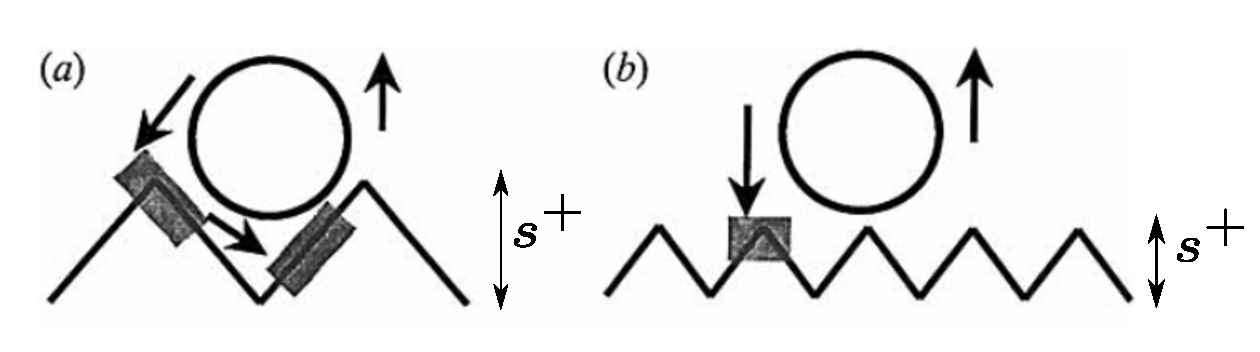
\includegraphics[width=0.7\linewidth]{chapter_1/riblets1}
	\caption{Two different size of riblets are represented interacting with a sublayer vortex. In grey is it represented the areas where the friction is important; clearly when the size of two is comparable (as the left picture) the surface experience a larger friction and the performance is lowered. Image from \citet{choi1993direct}}
	\label{fig:riblets_schem}
\end{figure}

The slope $m_s$ of the curve \ref{fig:riblets_perf} can be predicted by linear stability theory or by means of empirical correlations as in \citet{garcia2011hydrodynamic}.

Computing the performance of such surfaces can be expensive since the most reliable quantitative theory for such problems are DNS simulations or experiments.
There is only one other theory, besides the already cited expensive ones, that use the concept of of \textit{protusion height} showed in \ref{fig:riblets1} to correlates the shape of the protusion to the drag reduction \citet{luchini1991resistance}.
The \textit{protusion height} is defined as the vertical distance between the riblet top ridge and point of zero velocity extrapolated from the constant velocity gradient outside above the protusions.
It seems that especially the difference of protusion heights computed from the streamwise $h_{ps}$ and cross-flow flow $h_{pc}$ correlates very well with the drag reduction, and the two quantities can be computed with a simple Stokes problem over the local geometry of the grooves.

Another very impressive characteristic is that the performance are robust in off-design, such as the yaw (misalignment between the flow and the riblets ridges) and tip erosion of the ridges \citet{garcia2011drag}.

But still besides some very specific application, such as  sailing competitions in which the hulls of the USA challengers in the America’s Cup 1987 and 2010 were fitted with riblets, the massive utilization of this technology is still in question.
Since the riblets size need to be very little, producing such surfaces in a larger area like the roof of a car or the wing of an airplane can be an issue for a routine use.

Riblets like surface has been observed in nature for many years, for example \citet{Martin2016riblets} found out that skimmer birds (Rynchops) have riblets like grooves in their beak, since they fly with it under the surface of the water to catch fishes.
But, as already introduced, the most clear example of such natural surfaces are shark skin.
In his review \citet{dean2010shark} present the status of the shape optimization that has been done on the riblets trying to mimic the typical sawthoot shape seen in shark skin, showing that improvements of such geometries over the classical ones has yet to be proven.
Shape optimization on riblets geometry has been studied also by \citet{bechert1997experiments} finding that the drag reduction can be improved very little just working on the geometry even though a few $\%$ can be gained.

There is in fact some controversial result in literature that state that surfaces with actual shark skin replica can indeed increase drag.
\citet{boomsma2016direct} for example perform some simulations on actual shark skin denticles using the immersed boundary method; he find that in some configuration 
the actual drag increase up to $40\%$, but even though the numbers are probably too large (it is know that the immersed boundary method can generate large errors in force computation especially in high Reynolds number flows), this can prove that the shark skin does not work with the same mechanism as riblets.

In fact \citet{bechert1997natural} had already tested such geometries in his experiments. 
He builds a synthetic surface made by artificial shark denticles posed on top of spings and he measure that even with the introduction of the surface elasticity the actual drag was increasing.
however the authors pinpoints that the actual shark flow regime is nothing at all as steady as the experiments that he performed, and he speculates that the excellent swimming performance of the shark came from the separation control that flexible denticles can increase in the periodic oscillating flow that the swimming generate.

Experiment using DPIV on a NACA covered with actual skin samples of "Isurus oxyrinchus" mako shark, has been performed by \citet{lang2014SharkControl}, confirming that the flexibility of sharks denticles perform as a passive flow control in order to avoid early separation.
In fact the experiments proves that for angles of attack larger than $15^{\circ}$ the flow reversal is almost completely avoided.
The same author introduce the importance in the different geometries of the denticles in different part of the body that obviously experience different flow condition,
\citet{motta2012Shark} perform a detailed collection of flexibility and scale measurement of different shark species that can be valuable for future studies.

Swimming experiment from \cite{Oeffner785}, who used a flat plate covered with real shark skin, also confirm the previous flow control mechanism and also make some conjectures about possible thrust enhancing controlled by the same movable scale that can move away the leading edge vortex.

Also \citet{itoh2006turbulent} shows that movable rugosities can outperform riblets, the authors in fact measure the drag reduction of a seal fur (that present fibrous movable surface) against a riblet surface in an experimental channel; its results are show in figure \ref{fig:seal}.

\begin{figure}[h]
\centering
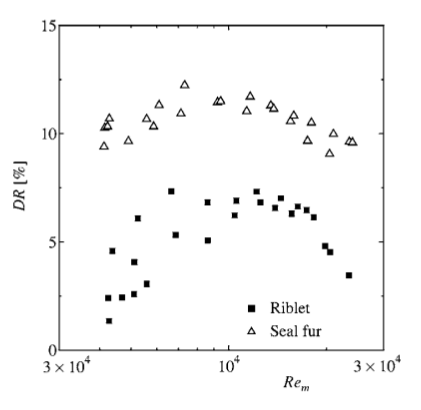
\includegraphics[width=0.5\linewidth]{chapter_1/seal}
\caption{$DR \% = \dfrac{ \Delta \tau}{\tau_{0}} \%$ Image from \citet{itoh2006turbulent}.}
\label{fig:seal}
\end{figure}


Compliant surfaces can in fact move accordingly to the surface pressure gradients along the boundary layer and so respond to the pressure fluctuation over the surface itself.
This mechanism is already know to be beneficial to delay the transition to turbulence and many authors have presented theoretical and experimental evidence on the effectiveness of this solution \cite{carpenter1990status}, \cite{bushnell1977effect}.

So we have seen that to reduce turbulent skin-friction drag riblets and natural surfaces uses various mechanism such as: sublayer vortices interaction, compliance and separation control.
Such solution have proven to be effective in some cases but they are related mostly in reducing the viscous component of the total drag.
In the next section we will introduce another class of solution that try to act instead on the pressure component.


\subsection{Permeable surfaces}

Permeable surface has been proposed to exploit even further the mechanism explained above using riblets.
There is some experimental evidence that in laminar cases the generation of some \textit{slip velocity}, at the interface between the permeable surface with the fluid , can decrease the friction drag \citet{beavers1967boundary}.
However in the turbulent case it seems that the instabilities developing at the interface can cause an increase in drag up to $40\%$ \citet{jimenez2001turbulent}, \citet{breugem2006influence}; this last mechanism will be further exploited in the section \ref{sec:stability}.
Is important to pinpoint that the permeable surface cited in the above references were all rigid.

The resistance pressure contribution is usually the most significant one in bluff bodies applications, and even in highly streamlined body it is around $10\%$ of the total drag.
Researchers have tried to find a way to modify the pressure distribution around a bluff body to reduce the associated resistance, and also dump the force oscillation on the body (drag and/or lift).

The pressure drag on a bluff body depends mostly on the difference between the low pressure on the rear part of the body, where there is usually a separated flow region, and the high pressure in the forward part.
This idea is sketched in figure \ref{fig:pressure_dist} where two different pressure distribution are shown; the black one represent the classical solid body, and the green one is the one with a porous layer at the back of the body.

\begin{figure}[h]
	\centering
	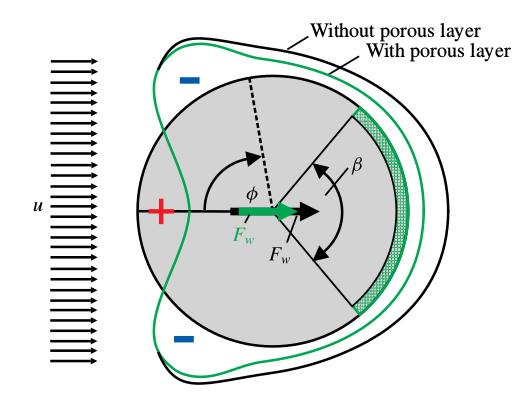
\includegraphics[width=0.4\linewidth]{chapter_1/pressure_dist}
	\caption{Diagram showing an example of pressure distribution around a cylinder for a viscous flow. The black line is the angular distribution as a solid body, the green one is the modified pressure in presence of a porous layer at the rear part. Image from \citet{klausmann2017drag}}
	\label{fig:pressure_dist}
\end{figure}

The favorable increase in the back pressure is due to the low speed laminar flow in the porous media that is ejected in the back region where the separation take place.
Even in very high speed turbulent flow the fluid inside permeable surface exhibit a very high energy loss due to the strong dissipation that the medium provide, resulting so in a low speed flow ejected downstream of the body.

The instability around a cylinder is due to the shear layer that forms in the top part of the body when the flow start to decelerate.
This shear layer exhibit a Kelvin–Helmeholtz type instability that develop in the classical Von-Karman wake.
The permeable interface, producing a slip velocity, can modify the boundary layer that develops above it and with that produce less shear and vorticity.

This two hypothetical mechanisms has been tested numerically numerically by multiple authors: \citet{bruneau2004passive}, \citet{bruneau2008numerical}, \citet{bhattacharyya2011reduction}, \citet{naito2012numerical}, \citet{mimeau2017passive}.
In their work they have add a porous layer to some classical two dimensional bluff bodies (cylinder, square cylinder, Ahmed body section, 3D hemisphere)and performed laminar and turbulent simulation for the flow around such bodies.

These works show some very strong result on multiple quantities, like: decrease of entstrophy, lower root mean square of the lift signal, drag reduction, regularization of the wake and lower pressure gradients; even if the porous medium is always rigid in their case.
An example is shown in figure \ref{fig:porous_cylinder} where the flow field downstream to a square cylinder is computed in a turbulent case; the picture show how the porous layer strongly regularize the wake.

\begin{figure}[h]
	\centering
	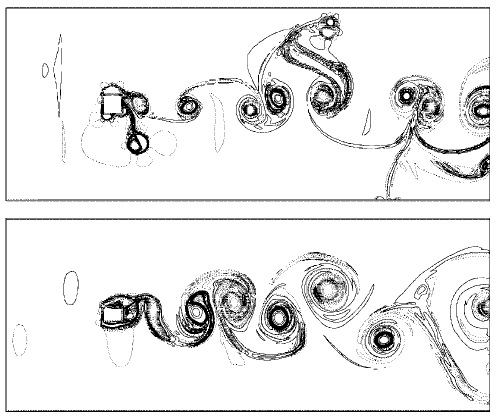
\includegraphics[width=0.7\linewidth]{chapter_1/cylinder_porous}
	\caption{Square cylinder vorticity countour for $Re=30000$. Top: solid case. Bottom: porous case with layer extension $h=10\% D$.}
	\label{fig:porous_cylinder}
\end{figure}


It seems from the previous works that the porous medium parameters, like the permeability (resistance) or its vertical extension, have important effects on the results.
They seems to agree (at least qualitatively) that increasing too the porous medium extension over a certain limit is not beneficial, and they also show that the resistance of the medium in order to be effective should not be excessive (medium to high porosity are the best).

In all these work we observe a reduced pressure drop between the front and the rear of the body, a reduced drag, delays in the vortex shedding in the laminar case and regularization on both the frequency and the amplitude of shedded vorticies oscillations.

These early work show very optimistic numbers but they should be taken with some care; only few cases are three-dimensional, and they all use a modeling approach for the porous medium based on a simplified version of the VANS (volume average Navier-Stokes equations, see section \ref{sec:vans}) without performing any validation of the method, and sometimes they use the equations outside their field of validity (there is some discussion in the scientific community in using such methods for highly turbulent flows).

The lack of validation reflect the fact that reliable experiment of such porous coatings are almost non existent in literature.
They also do not agree on the methods used to compute the forces \citet{caltagirone1994interaction}?? SHOW HERE THE GOOD METHOD ? MAYBE IN THE VANS SECTION...


\citet{favier2009passive} use a different numerical method that includes the dynamic of a moving porous medium made of fibers at the back of a cylinder.
Their results in a laminar flow case agree with the results on the stabilization of the wake and show some more realistic values of drag reduction, about $15\%$.
The difficulties in this model is in the medium dynamic, since it introduce many mechanical parameters that are not easy to identify for natural surfaces.

A similar model to the previous one has been used by \citet{venkataraman2012numerical}; the authors applied a movable porous coating in the top part of naca airfoil.
In this case the synchronization between the oscillations of the structures and the natural frequency of the fluid is responsible for the pressure distribution modification.
They have shown the robustness of this solution in a wide range of angle of attack, in the best case they have found some lift enchantment and regularization and a drag reduction has been measured to be on the order of $10\%$.

Later on \citet{rosti2017pelskin} works on a similar configuration with only one movable flap on the low pressure side of airfoil; the results both numerical and experimental qualitatively agree (on the flow mechanism) with the results in the complete porous case.


WHEN IT WILL BE PUBLISHED SHOW SOME RESULTS ON THE 3D SPHERE USING HOMOGENIZATION \citet{zampogna2017new}

The are very few experiment in literature on this porous coatings, but they all seems to show less promising numbers when  dealing with drag reduction.

For example \citet{heenan1998passive} perform an experiment in which he take a backward facing step with a porous insert in the re-circulation region.
His measurement show a $13\%$ decrease of the peak of pressure at the wall and a relocation of the detachment point further downstream.
Also depending on the length of the porous insert a maximum of $9\%$ of drag reduction was also observed.
The effect of adding a porous surface in this case was to limit the pressure fluctuations that causes the re-circulation bubble unsteadiness.

Later \citet{klausmann2017drag} study a 3D cylinder with a porous insert in the back; the authors use a wind tunnel testing with pressure measurements around the body and particle image velocimetry (PIV) flow capture.
Their results confirms that the porous layer on the leeward side increase of pressure in that zone, causing the reduction of drag.
The drag reduction measured to be around $10\%$ over various Reynolds number in the fully developped turbulence range, but it can be more sensible to the geometrical parameters of the medium as the position and its size.
At our knowledge this is the first example of actual measurements of flow quantities using PIV, that can later be used to perform some validation on different numerical models.

Some other experimental data can be found in the case of flow over aquatic canopies \citet{zhang2011exchange}, \citet{segalini2011experimental}, even though the published data is limited and the problem in this case has also a free surface that increase the difficulty of the problem and limits the possible use as validation.

From this section the main physical mechanism that tied to permeable surfaces has been introduced but the different approaches in literature seems to be discordant in the predicted values of some fundamental items such as the forces.
Is it clear that the scientific community need much more experimental data in order to develop new and improved numerical and theoretical models for such permeable coatings.


\section{Models for flows through porous surfaces}
\subsection{Drag that is function of the canopy depth (canopy flow, flow vegetation)}
\subsection{Porous media approach through homogenization}
\subsubsection{VANS}
\label{sec:vans}

Penalization method \citet{angot1999penalization} used in\cite{bruneau2004passive} \cite{bruneau2008numerical} \cite{bruneau2010coupling}...

\subsubsection{Multiple scales}

\section{Stability of flow over permeable surfaces (monami and honami)}
\label{sec:stability}

\citet{finnigan2000turbulence} \citet{jimenez2001turbulent}

\subsection{Stability theory generalities}
\subsection{Monami Honami}